% !TeX root = ../main.tex
\documentclass[../main.tex]{subfiles}
\begin{document}
    \section{Konkrete Zahlen}
    Hier werden die hergeleiteten Formeln angewendet, um konkrete Zahlen zu erhalten.
    Um einen Maßstab zu sehen werden jeweils ein Erdenjahr (365 Tage), ein Marsjahr (780 Tage) und ein Jupiterjahr (4330 Tage) gezeigt.

    \subsection{Wahrscheinlichkeit der ersten Kollision}

    Mithilfe der Formel \ref{num.pleq} wird die Wahrscheinlichkeiten dafür berechnet, dass $X \leq k$ ist. $X$ ist hierbei der
    Zeitpunkt der 1. Kollision.
    Mit der Formel \ref{num.peq} wird die Wahrscheinlichkeit errechnet das die Kollision bei $k$ stattfindet.

    \begin{equation}
        \mathbb{P}(X \leq k) \approx 1 - e^{- \frac{k(k-1)}{2n}}
        \label{num.pleq}
    \end{equation}

    \begin{equation}
        \mathbb{P}(X = k) \approx \frac{(k-1)}{n} \cdot e^{- \frac{(k-1)^2}{2n}}
        \label{num.peq}
    \end{equation}

    \subsubsection{$\mathbb{P}(X \leq k)$}

    \textbf{Erde}

    \begin{table}[h]
        \centering
        \begin{tabular}{|l|l|l|l|}
            \hline
            $k$ & $\mathbb{P}(X_{n}) \leq k)$ & $k$ & $\mathbb{P}(X_{n}) \leq k)$ \\ \hline
            0   & 0,001                       & 40  & 0,876                       \\
            10  & 0,105                       & 50  & 0,963                       \\
            20  & 0,390                       & 60  & 0,992                       \\
            30  & 0,684                       & 70  & 0,999                       \\ \hline
        \end{tabular}
        \caption{\label{num.tpe} Wahrscheinlichkeit für die erste Kollision nach höchstens $k$ Personen auf der Erde}
    \end{table}

    \begin{figure}[h]
        \begin{center}
            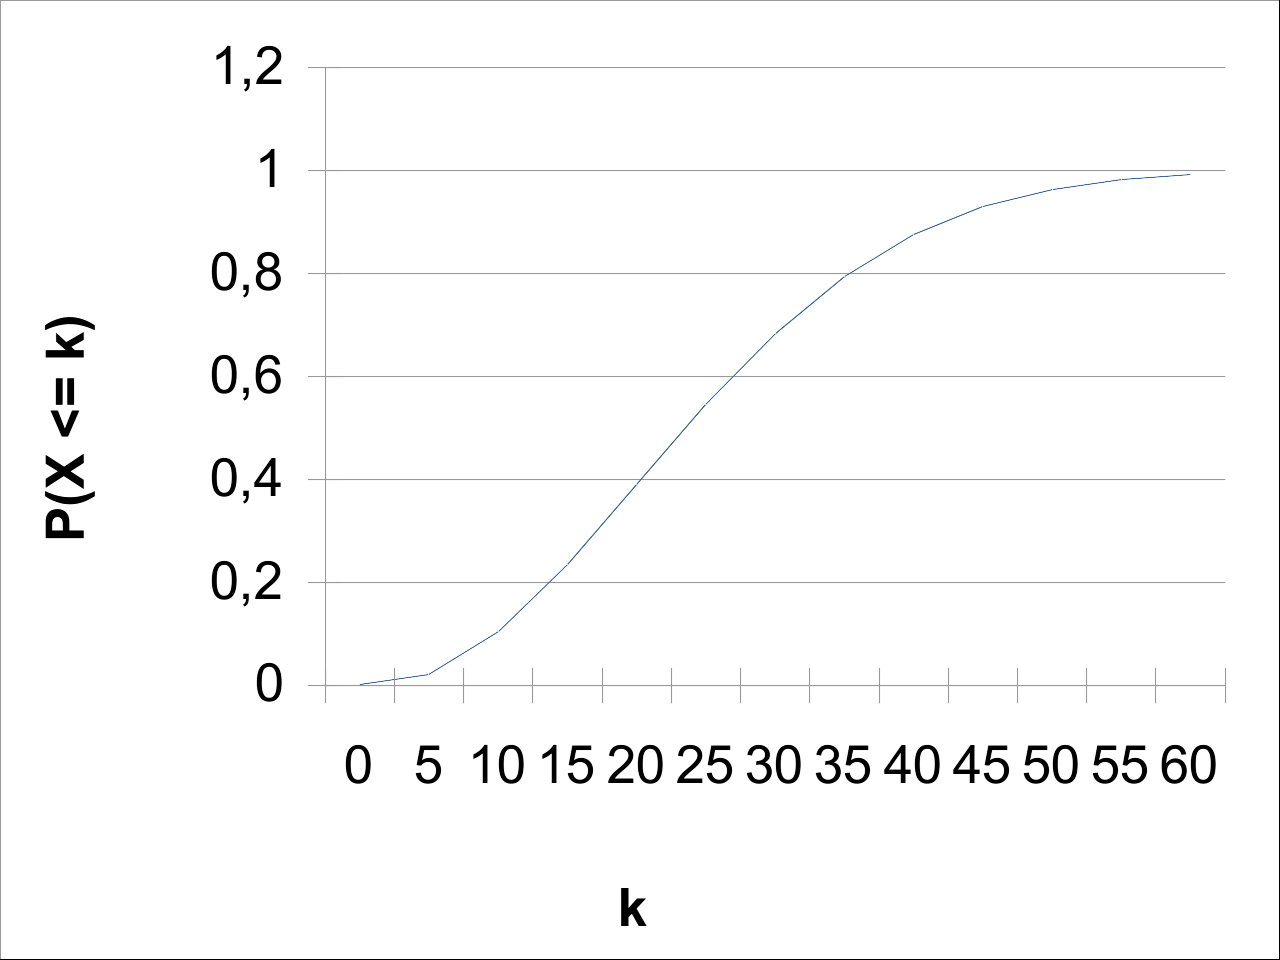
\includegraphics[width=0.7\textwidth]{../graphics/perde.png}
            % qerde.png: 1280x960 px, 72dpi, 45.16x33.87 cm, bb=0 0 1280 960
        \end{center}
        \caption{\label{num.fpe} Wahrscheinlichkeit für den ersten gleichen Geburtstag nach höchstens $k$ Ziehungen}
    \end{figure}


    \textbf{Mars}

    \begin{table}[h]
        \centering
        \begin{tabular}{|l|l|l|l|}
            \hline
            $k$ & $\mathbb{P}(X_{n} \leq k)$ & $k$ & $\mathbb{P}(X_{n} \leq k)$ \\ \hline
            0   & 0,001                      & 60  & 0,893                      \\
            15  & 0,118                      & 75  & 0,970                      \\
            30  & 0,417                      & 90  & 0,994                      \\
            45  & 0,711                      &     &                            \\ \hline
        \end{tabular}
        \caption{\label{num.tpm} Wahrscheinlichkeit für die erste Kollision nach höchstens $k$ Personen auf dem Mars}
    \end{table}

    \textbf{Jupiter}

    \begin{table}[h]
        \centering
        \begin{tabular}{|l|l|l|l|}
            \hline
            $k$ & $\mathbb{P}(X_{n} \leq k)$ & $k$ & $\mathbb{P}(X_{n} \leq k)$ \\ \hline
            0   & 0                          & 120 & 0,805                      \\
            30  & 0,093                      & 150 & 0,923                      \\
            60  & 0,331                      & 180 & 0,975                      \\
            90  & 0,599                      & 210 & 0,994                      \\ \hline
        \end{tabular}
        \caption{\label{num.tpj} Wahrscheinlichkeit für die erste Kollision nach höchstens $k$ Personen auf dem Jupiter}
    \end{table}

    \subsubsection{$P(X = k)$}

    \textbf{Erde}

    \begin{table}[h]
        \centering
        \begin{tabular}{|l|l|l|l|l|l|}
            \hline
            $k$ & $\mathbb{P}(X_{n} = k)$ & $k$ & $\mathbb{P}(X_{n} = k)$ & $k$ & $\mathbb{P}(X_{n} = k)$ \\ \hline
            5   & 0,011                   & 25  & 0,030                   & 45  & 0,009                   \\
            10  & 0,022                   & 30  & 0,025                   & 50  & 0,005                   \\
            15  & 0,029                   & 35  & 0,019                   & 55  & 0,003                   \\
            20  & 0,032                   & 40  & 0,013                   & 60  & 0,001                   \\ \hline
        \end{tabular}
        \caption{\label{num.tpeqe} Wahrscheinlichkeit für die erste Kollision bei der $k$-ten Person}
    \end{table}

    \begin{figure}[h]
        \begin{center}
            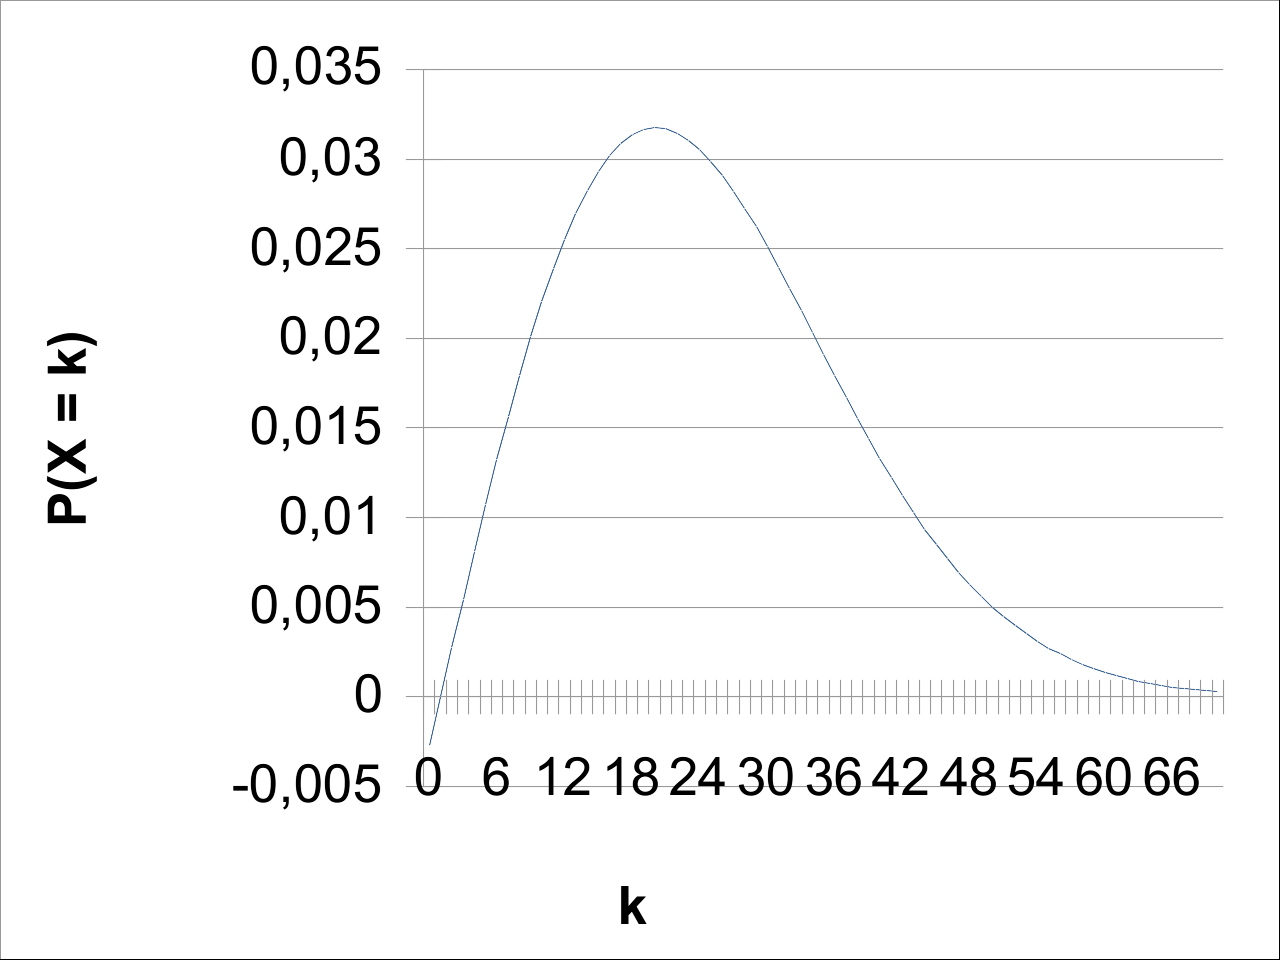
\includegraphics[width=0.7\textwidth]{../graphics/peq.png}
            % peq.png: 1280x960 px, 72dpi, 45.16x33.87 cm, bb=0 0 1280 960
        \end{center}
        \caption{\label{num.fpeqe} Wahrscheinlichkeit für die erste Kollision bei der $k$-ten Person}
    \end{figure}



    Die höchste Wahrscheinlichkeit das die erste Kollision genau bei $k$ auftritt, liegt auf der Erde bei \bm{$\sim 20,105$} (zu sehen auf Grafik \ref{num.fpeqe}), auf dem Mars bei \bm{$\sim 28,928$} und auf dem Jupiter bei \bm{$\sim 66,803$}, also jeweils bei \bm{$1 + \sqrt{n}$}.

    \subsection{Erwartungswerte}

    Der Erwartungswert für die erste Kollision wird über die Formel \ref{num.exp} errechnet.

    \begin{equation}
        E(X) \approx 1 + \sqrt{\frac{1}{2} \pi n}
        \label{num.exp}
    \end{equation}

    Für die verschiedenen Planeten kommen dabei folgende Werte heraus:

    \begin{center}
        \begin{tabular}{|l|l|}
            \hline
            \textbf{Planet} & \textbf{Erwartungswert} \\ \hline
            Erde            & 24,945                  \\ \hline
            Mars            & 36,003                  \\ \hline
            Jupiter         & 83,472                  \\ \hline
        \end{tabular}
    \end{center}

    \subsection{Quantile}

    Die Quantile für die erste Kollision werden über die Formel \ref{num.q} berechnet.

    \begin{equation}
        q_{\alpha} \approx 1 + \sqrt{2n \cdot ln(1-\alpha)}
        \label{num.q}
    \end{equation}

    \begin{table}[h]
        \centering
        \begin{tabular}{|l|l|l|l|}
            \hline
            $\alpha$      & $q_{\alpha}$ Erde & $q_{\alpha}$ Mars & $q_{\alpha}$ Jupiter \\ \hline
            $\frac{1}{4}$ & 15,492            & 22,185            & 50,913               \\
            $\frac{1}{2}$ & 23,494            & 33,883            & 78,477               \\
            $\frac{3}{4}$ & 32,812            & 47,504            & 110,569              \\ \hline
        \end{tabular}
    \end{table}


\end{document}
